
%----------------------------------------------------------------------------------------
%	Lecture 14
%----------------------------------------------------------------------------------------

\chapter{Change of Variables}

\bigbreak

\section{Finding the area of ellipse}

Let the length of x-axis and y-axis of the ellipse be $a$ and $b$, respectively.
The equation of the ellipse is 
$$ \left( \frac{x}{a} \right)^2 + \left( \frac{y}{b} \right)^2 = 1 $$

\begin{figure}[ht!]
    \centering
    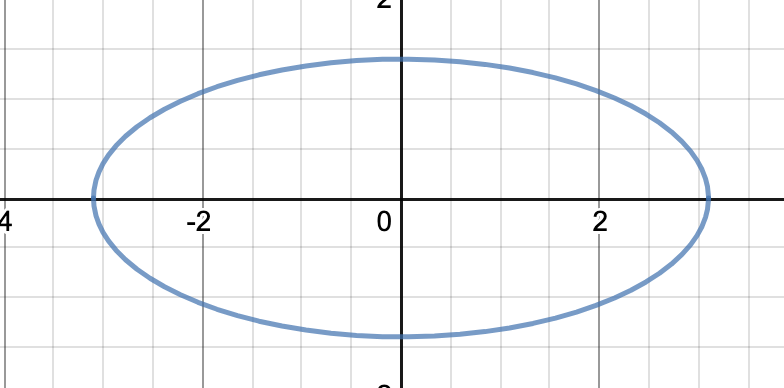
\includegraphics[scale=0.5]{./images/lecture_14_figure_1.png}
    \caption{Graph of the ellipse}
\end{figure}

Let's find the area of the ellipse as a double integral.
Our region is the area inside the ellipse. So we want to find the area of that region.
But the bounds of that region are difficult.
Maybe we can convert it into a cirlce. So for that we'll set $x = au$ and $y = bv$.
And we'll try to redo the integral in terms of $u$ and $v$.
Our region becomes $u^2 + v^2 \leq 1$. And we have $dx = adu$ and $dy = bdv$.

$$
Area = \iint dx dy = \iint_{u^2+v^2 \leq 1} ab du dv = ab \iint_{u^2+v^2 \leq 1} du dv = \pi a b 
$$

Here the final integral is just the area of a circle with unit radius which we know to be $\pi$.


\section{Change of Variables}

In general, we need to find the scaling factor for $dA$ when we change from $x, y$ to $u, v$.
Let's say $u = 3x - 2y$ and $v = x + y$, then we need to find the relation between $dA = dx dy$ and $dA' = du dv$.
$\Delta A$ is a rectangle in the XY-coordinates but it might become a parallelogram in UV-coordinates depending upon the tranformation.

Area scaling factor in a linear transformation does not depend on the choice of rectangle.
So the exchange rate of $u, v$ and $x, y$ will be the same everywhere.

\pagebreak

Let's take a unit square with opposite vertices at $(0, 0)$ and $(1, 1)$.

\begin{figure}[ht!]
    \centering
    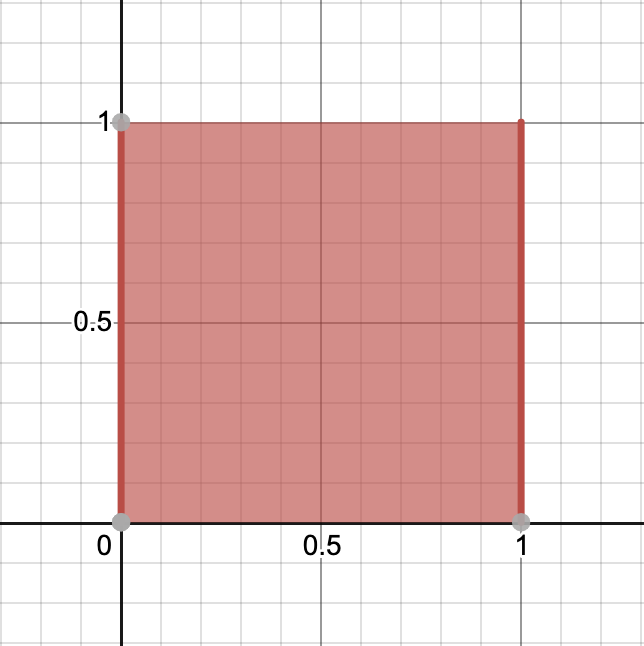
\includegraphics[scale=0.5]{./images/lecture_14_figure_2.png}
    \caption{Graph of the unit square}
\end{figure}

If we transform the endpoints according to the above transform then we'll get the endpoints
at $(0,0) \to (0,0)$, $(1, 0) \to (3, 1)$, $(0, 1) \to (-2, 1)$ and $(1, 1) \to (1, 2)$.

\begin{figure}[ht!]
    \centering
    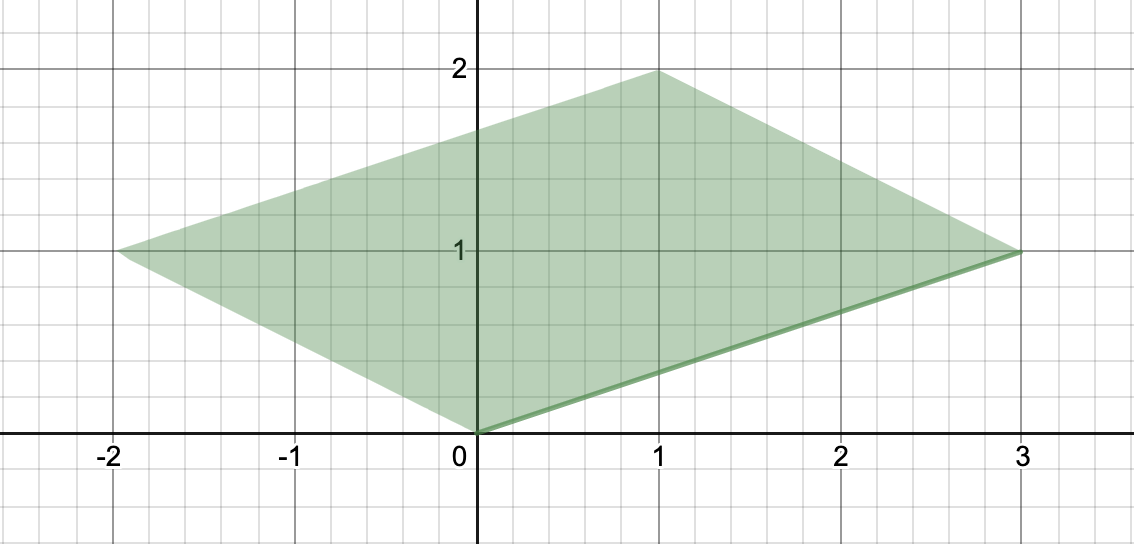
\includegraphics[scale=0.5]{./images/lecture_14_figure_3.png}
    \caption{Transformed square}
\end{figure}

If we find the are of the parallelogram gram we'll get, 
$$
A' = |(\ij{3}{1}) \times (\ij{-2}{1})| = |3 - (-2)| = 5
$$

Thus, the scaling factor is $5$. 

That tells us that for any rectangle are is multiplied by $5$.
So $ dA' = 5 dA \rightarrow du dv = 5 dx dy $

Thus, \ilds{ \iint f(x, y) dx dy \rightarrow \iint f(u, v) \frac{1}{5} du dv }

Since we did a linear transform the scaling factor is constant. 
But if we did a change of variables which is non-linear then we'll get a formula for the scaling factor which will depend on $u, v$.

\subsection{General Case}

In general, $u = u(x, y)$ and $v = v(x, y)$ so by linear approximation we have $du = u_x dx u_y dy$ and $dv = v_x dx + v_y dy$. 
So for a general rectangle in XY-plane there is a corresponding parallelogram in th e UV-plane and its area will depend on the rate of change of $u, v$ with respect to $x, y$.

$$
\begin{bmatrix}
    du \\ dv \\
\end{bmatrix}
=
\begin{bmatrix}
    u_x & u_y \\
    v_x & v_y \\
\end{bmatrix}
\begin{bmatrix}
    dx \\ dy \\
\end{bmatrix}
$$

So if we move in the direction $(dx, 0)$ then in UV-plane the new point will move by $(u_x dx, v_x dx)$.
And it we move in the direction $(0, dy)$ then point in UV-plane will move by $(u_y dy, v_y dy)$.
So the area of the parallelogram will be the determinant of these vectors.

{\bf Note:} We cannot just multiple $du$ and $dv$ in terms of $dx$ and $dy$ as it forms a parallelogram. 
Thus, we need the cross product.

So the new area is $|(u_x v_y - v_x u_y)| dx dy = |det(J)| dx dy$.
Here $J$ is the matrix of the partial derivatives given above and it is called the Jacobian of the tranformation.
We denote it by,

$$
J = \px{(u, v)}{(x, y)} = 
\begin{vmatrix}
    \px{u}{x} & \px{u}{y} \\
    \px{v}{x} & \px{v}{y} \\    
\end{vmatrix}
$$
$$
du dv = | J | dx dy
$$

So the scaling factor is the absolute value of the Jacobian.

{\bf Example: } For polar coordinates we know that, $dx dy = r dr d\theta$.
The change of variables is $x = r \cos \theta$ and $y = r \sin \theta$.

\begin{align*}
    dx dy 
        & = \px{(x, y)}{(r, \theta)} dr d\theta \\
        & = \begin{vmatrix}
            \px{x}{r} & \px{x}{\theta} \\
            \px{y}{r} & \px{y}{\theta} \\
        \end{vmatrix} dr d\theta \\
        & = \begin{vmatrix}
            \cos \theta & - r \sin \theta \\
            \sin \theta & r \cos \theta \\
        \end{vmatrix} dr d\theta \\
        & = (r \cos^2 \theta + r \sin^2 \theta) dr d\theta \\
    dx dy & = r dr d\theta
\end{align*}


\subsection{Inverse Jacobian}

There are two kinds of Jacobian you can compute. But these are inverses of each other.
That is multiplying them will give you the identity matrix $I$.
\begin{align*}
    \px{(x, y)}{(u, v)} \cdot \px{(u, v)}{(x, y)} = I \\
    \begin{bmatrix}
        x_u & x_v \\
        y_u & y_v
    \end{bmatrix}
    \cdot
    \begin{bmatrix}
        u_x & u_y \\
        v_x & v_y
    \end{bmatrix} = I \\
    \begin{bmatrix}
        (x_u u_x + x_v + v_x) & (x_u u_y + x_v v_y) \\
        (y_u u_x + y_v v_x) & (y_u u_y + y_v v_y) \\
    \end{bmatrix} = I \\
    \begin{bmatrix}
        \px{x}{x} & \px{x}{y} \\
        \px{y}{x} & \px{y}{y}
    \end{bmatrix} = I \\
\end{align*}

Since, $x$ and $y$ are indepedent variables so $\px{y}{x}$ and $\px{x}{y}$ are zero.
Thus, proved.


{\bf Example : } Let's say we want to compute \ilds{ \int_0^1 \int_0^1 x^2y dx dy }
Let $u = x$ and $v = xy$.

First, we'll find the Jacobian.
$$
\px{(u, v)}{(x, y)}  = 
    \begin{bmatrix}
        1 & 0 \\
        y & x \\
    \end{bmatrix} 
    = x
$$

So, we have $du dv = x dx dy \Rightarrow dx dy = (1/u) du dv$ as $ u = x $.

So our integration becomes,
$$ \iint uv \frac{1}{u} du dv = \iint v du dv $$

Finally, we want to find out the bounds of integration.
Let's say we want to integrate with respect to $u$ first so we need to keep $v$ constant.
But $v = xy$ so keeping $xy = constant$ we get the curve shown below.

\begin{figure}[ht!]
    \centering
    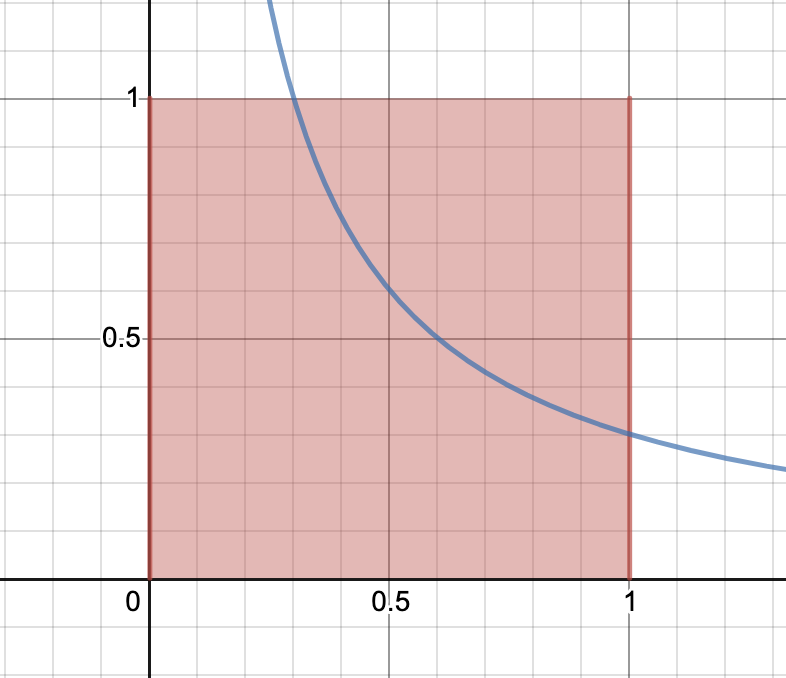
\includegraphics[scale=0.5]{./images/lecture_14_figure_4.png}
    \caption{Transformed square}
\end{figure}

\pagebreak

Now, we need to find the bounds on $u$ along this curve starting at the point where it enters the region
and ending at the point where it leaves the region.
Since $u = x$ we only need to calculate the $x$ coordinate of those points.
At the enterance, $y = 1$ but \ilds{y = \frac{v}{x} = \frac{v}{u}} so our equation along the enterance is $u = v$.
At the exit, $x = 1$ so  $u = 1$.

Now for the bounds for $v$, the smallest value of $xy$ is $0$ and it goes up to $1$.
So our integral becomes, 

$$
\int_0^1 \int_v^1 v du dv  
    = \int_0^1 v(1-v) dv 
    = \int_0^1 v - v^2 dv 
    = \frac{1}{2} - \frac{1}{3} 
    = \frac{1}{6}
$$

This is not the ideal method. You can also create a diagram in the UV-plane to find the bounds.
It depends on the problem which will be easier.
